% -*- mode: fundamental -*-

% ****************************************************************

\chapter{BSV: Combinational circuits for the RISC-V step functions}

\markboth{Ch \arabic{chapter}: Combinational functions (DRAFT)}{\copyrightnotice}

\setcounter{page}{1}
% \renewcommand{\thepage}{\arabic{page}}
\renewcommand{\thepage}{\arabic{chapter}-\arabic{page}}

\label{ch_Combo_Circuits}

% ****************************************************************

\section{Introduction}

It is useful to start with the Decode step of
Figure~\ref{Fig_Instr_Exec} because it involves bit-vectors,
operations on bit-vectors, conditionals to classify instructions into
classes, and \verb|enum| types to name and encode instruction classes.

The inputs to the Decode step as depicted in
Figure~\ref{Fig_Instr_Exec} are:

\begin{tightlist}

 \item A 32-bit piece of data---a RISC-V instruction---that has become
 available by reading it from memory at the PC address.\footnote{When
 implementing the so-called ``C'' RISC-V ISA extension (``compressed
 instructions''), instructions can also be 16-bits, but we
 ignore that for now.}

 \item Any additional information passed on from the Fetch step.

\end{tightlist}

The outputs of the Decode step have information needed by the next
step (Register-Read and Dispatch).  For a RISC-V instruction, useful
information includes:

\begin{tightlist}

 \item Was the Fetch itself successful, or did it encounter a memory
   error; if so, what kind of memory error?

 \item Is it a legal 32-bit instruction?

 \item If legal, what is its broad classification: Control (Branch or
   Jump)? Integer Arithmetic or Logic? Memory Access?  This will help
   in choosing the next step to which we must dispatch to execute the
   instruction.

 \item Does it have zero, one or two input registers?  If so, which
   ones?  This will help the next step in reading registers.

 \item Does it have zero or one output registers?  If so, which one?
   This will help the final Register Write step in writing back a
   value to a register.

\end{tightlist}

To compute these values, we need to examine ``slices'' of the 32-bit
instruction (``bit vector''), such as the 7-bit ``opcode'' slice, the
5-bit ``rs1'', ``rs2'' and ``rd'' slices, and so on.  We need to be
able to compare these slices to constants ({\eg} ``Is the opcode a
BRANCH opcode?'').  We need to do things conditionally, {\eg} if it is
a BRANCH instruction, then it has an rs1 and rs2 slice but no rd
slice, but if it is a JAL instruction it has an rd slice but no rs1 or
rs2.  Finally, as in all good programming languages, we'd need to be
able to package all this functionality inside a ``function'' with
clearly specified input(s) and output(s).  In the next several
sections---\ref{Sec_BSV_Bit_Vectors}, \ref{Sec_BSV_Boolean_values},
\ref{BSV_functions}, \ref{BSV_Combo_Circuits_if_then_else}, ---we will
learn the BSV concepts needed to code these ideas.

% ****************************************************************

\section{Bit Vectors}

\label{Sec_BSV_Bit_Vectors}

\index{BSV!Bit Vectors}
\index{BSV!Types!{\tt Bit\#(n)}}

In BSV, as in many programming languages, every value has a
\emph{type}.  The simplest, and lowest-level type in BSV is the
bit-vector (a vector made up of a particular number bits).  Later we
will see that in BSV one can define more abstract types such as
integers, booleans, vectors and arrays, lists, structs (records),
tagged unions (algebraic types), trees, and so on.  However,
ultimately, any such value is represented in hardware as a bit-vector.

The BSV statement:

{\small
\begin{Verbatim}[frame=single, numbers=left]
   Bit #(32) pc_val;
\end{Verbatim}
}

declares the identifier \verb|pc_val| to have the type
\verb|Bit#(32)|, {\ie} a bit-vector of 32 bits.
The general syntax is similar to C or Verilog:
\begin{quote}
\emph{type} \emph{identifier};
\end{quote}

The BSC type \verb|Bit#(32)| is roughly equivalent to the C type
\verb|uint32_t|.  Unlike C, where only a few sizes are available, all
multiples of 8 bits--- (\verb|uint8_t|, \verb|uint16_t|,
\verb|uint32_t| and \verb|uint64_t|)---bit-vectors in BSV can have any
size (\verb|Bit#(3)|, \verb|Bit#(51)|, \verb|Bit#(512)|, ...).

The bits in a BSV bit-vector of size $n$ are indexed from $n-1$
(most-significant bit) to 0 (least-significant bit).  You can extract
a \emph{slice} of a bit-vector using usual Verilog notation:

\index{BSV!Bit Vectors!slices of}

{\small
\begin{Verbatim}[frame=single, numbers=left]
   Bit #(32) pc_val;
   Bit #(12) page_offset = pc_val [11:0];
\end{Verbatim}
}

In the second line, we extract 12 bits of \verb|pc_val| to get a
bit-vector of size 12.  BSV is \emph{strongly typed} with respect to
sizes, {\ie} it is very strict about matching sizes.  For example,
this statement:

{\small
\begin{Verbatim}[frame=single, numbers=left]
   Bit #(12) page_offset = pc_val [10:0];
\end{Verbatim}
}

will be reported as a type-error by the \emph{bsc} compiler because
the slice-expression on the right-hand side has type \verb|Bit#(11)|
which does not match the declared type \verb|Bit#(12)|.

% ================================================================

\subsection{Built-in Operators on Bit Vectors}

\label{Bit_Vector_Ops}

BSV bit-vectors can be compared for equality and inequality.  BSV
bit-vectors are synonymous with unsigned integers, and so a number of
other operations are also available on bit-vectors.  Examples:

\index{BSV!Bit Vectors!operators on}
\index{BSV!Operators on Bit Vectors}

{\small
\begin{Verbatim}[frame=single, numbers=left]
   Bit #(12) x, a, b, c, d, e, f;

   // Comparison ops: result type is Bool
   if (a == b) ...;        // equality
   if (a != b) ...;        // not-equal to
   if (a < b) ...;         // less-than
   if (a <= b) ...;        // less-than-or-equal-to
   if (a > b) ...;         // greather-than
   if (a >= b) ...;        // greater-than-or-equal-to

   // Arithmetic ops: result type is Bit #(12)
   x = a + b - c * d;      // add, subtract, multiply

   // Bitwise logic ops: result type is Bit #(12)
   //   AND  OR   unary INVERT   XOR  XNOR  XNOR
   x = a &  b |     (~ c)         ^   d ^~ e ~^ f;

   // Shifts
   x = (a << 3) & (b >> 14);    // left- and right-shift
\end{Verbatim}
}

Please see the \emph{BSV Language Reference Guide}~\cite{BLang2000},
Section 10.3, ``Unary and binary operators'' for a full list of
available unary and binary operators.  Unlike Haskell, in BSV you
cannot define new unary or binary infix operators.

In such expressions, as usual bit-vector sizes must match exactly,
else we'll get a type error, {\eg} we cannot compare a
\verb|Bit#(12)| value with \verb|Bit#(11)| value.  Unlike C and
Verilog, BSV does not implicitly extend or truncate bit-vectors to
match sizes.

\index{BSV!Bit Vectors!{\tt truncate}}
\index{BSV!Bit Vectors!{\tt extend}}
\index{BSV!Bit Vectors!{\tt zeroExtend}}

Two functions are available to zero-extend and truncate bit-vectors.

{\small
\begin{Verbatim}[frame=single, numbers=left]
   Bit #(12) a;
   Bit #(10) b;
   b = a;                         // Type error: mismatched sizes
   a = b;                         // Type error: mismatched sizes
   b = truncate (a);              // Ok; truncates a to Bit #(10), then assigns
   a = zeroExtend (b);            // Ok; extends b to Bit #(12), then assigns
   if (a == zeroExtend (b)) ...   // Ok
   if (truncate (a) < b) ...      // Ok
\end{Verbatim}
}

The functions \verb|truncate()| and \verb|zeroExtend()| are
\emph{polymorphic} in that they will truncate/extend by the
appropriate amount as demanded by the context.

% ****************************************************************

\section{Integer types}

\label{BSV_ints}

\index{BSV!Integer types {\tt Bit}, {\tt Int}, {\tt UInt}, {\tt Integer}}
\index{BSV!Bit@{\tt Bit}!Integer type}
\index{BSV!Int@{\tt Int}!Integer type}
\index{BSV!UInt@{\tt UInt}!Unsigned integer type}
\index{BSV!UInt@{\tt Integer}!Unbounded (non-synthesizable) Integer type}

BSV has four integer types, written as follows:

{\small
\begin{Verbatim}[frame=single, numbers=left]
   Bit #(n)        // bit-vectors, bounded to n bits
   Int #(n)        // signed integers, bounded to n bits
   UInt #(n)       // unsigned integers, bounded to n bits
   Integer         // Mathematical integers (unbounded, no bit-width limit)
\end{Verbatim}
}

The most common type used in processor design (and possibly in all
hardware design) is \verb|Bit#(n)|.  \verb|UInt#(n)| can used to
represent unsigned integers, $n$ bits wide.  But since essentially the
same operators (\verb|+|, \verb|-|, \verb|&|, \verb'|', shifts, ...,
see Section~\ref{Bit_Vector_Ops}) are defined on both these types,
this author mostly uses \verb|Bit#(n)| for unsigned integers, and
rarely uses \verb|UInt#(n)|.

\verb|Int#(n)| is used whenever we need to represent negative numbers
and perform signed operations.  These are represented in bits in
hardware in ``2's complement'' representation (see
\url{https://en.wikipedia.org/wiki/Two%27s_complement}).

\verb|Integer| is used for true mathematical integers, {\ie} they are
unbounded, ranging from minus infinity to plus infinity (in practice,
limited by the amount of memory in your computer!).  Being unbounded,
they cannot be represented in any fixed-size hardware.  \verb|Integer|
is used only for compile-time integers, where we do not need to fix a
bound.

\index{BSV!Wraparound arithmetic for fixed-width integer types}

Fixed-width integer types all ``wrap-around''.  For example, if we add
1 to a \verb|Bit#(3)| value \verb|3'b_111|, the result will be
\verb|3'b_000|; if we subtract 1 from a \verb|Bit#(3)| value
\verb|3'b_000|, the result will be \verb|3'b_111|.

Note that all four type names begin with an upper-case letter.  This
is true of all types in BSV: type names and enumeration constants
begin with an upper-case letter, other identifiers begin with a
lower-case letter.  (See also
Section~\ref{BSV_Syntax_of_Identifiers}.)

% ****************************************************************

\section{Hexadecimal and Binary Notation for literal integers}

\label{BSV_hex_bin_literals}

\index{BSV!Literals!Hexadecimal integer notation}
\index{BSV!Literals!Binary integer notation}
\index{BSV!Hexadecimal notation for integer literals}
\index{BSV!Binary notation for integer literals}

BSV uses the same notation as Verilog and SystemVerilog for
hexadecimal and binary literal integers.  Some examples:

{\small
\begin{Verbatim}[frame=single, numbers=left]
3'b010            // Binary literal, 3 bits wide
7'b_110_0011      // Binary literal, 7 bits wide
5'h3              // Hex literal, 5 bits wide
32'h3             // Hex literal, 5 bits wide
32'h_efff_0f17    // Hex literal, 32 bits wide (an AUIPC instruction)
'h23              // Hex literal, context determines width
\end{Verbatim}
}

As these examples show, a hexadecimal or binary integer literal is
introduced by an optional bit-width, then a ``tick'' (single-quote)
character, and then the binary or hexadecimal digits for the number.
The character ``{\verb|_|}'' may be used freely to space out groups of
digits to improve readability for humans (the compiler ignores these
spacers).

The last line shows that we can omit the size prefix, in which case
the size will be inferred by the compiler from the context. For
example, if we had:

{\small
\begin{Verbatim}[frame=single, numbers=left]
   Bit #(32) pc_val = 'h_8000_0000;
\end{Verbatim}
}

then the literal is inferred to be 32 bits wide.

% ****************************************************************

\section{Boolean values}

\label{Sec_BSV_Boolean_values}

\index{BSV!{\tt Bool}}
\index{BSV!Types!{\tt Bool}}
\index{BSV!Bool@{\tt Bool}!operators on}

In BSV, \verb|Bool| is the type of a Boolean value. It has the usual
boolean operators \verb|&&| (Boolean/logical AND), \verb'||'
(Boolean/logical OR) and \verb|!| (Boolean/logical NOT).

% ================================================================

\subsection{Caution: {\tt Bool} and {\tt Bit\#(1)} are different types}

BSV is unlike languages like C and Python which are very loose about
what can be used as a boolean value.  For example in C, any non-zero
numeric value or pointer is considered ``True''.

In BSV, \verb|Bool| and \verb|Bit#(1)| are \emph{distinct} types,
{\ie} \emph{bsc}'s type-checking will complain if one is used where
the other is expected.  This is because not all \verb|Bit#(1)| values
are meaningful as Boolean values.

The Boolean/logical operators mentioned above (such as \verb|&&|)
operate on \verb|Bool| types and are distinct from the bit-wise logic
operators mentioned earlier (such as \verb|&|), which operate on
\verb|Bit#(n)| types.

Note that bitwise comparison operators, such as in the example
\verb|if (a <= b) ...| shown in Section~\ref{Sec_BSV_Bit_Vectors}
above, take \verb|Bit#(n)| arguments and produce \verb|Bool| results.

% ================================================================

\subsection{Example: recognizing legal RISC-V BRANCH instructions}

The RISC-V ISA has a family of six conditional-branch instructions.
Figure~\ref{Fig_Combo_BRANCH_instrs} is an excerpt from the Unprivileged ISA
specification document~\cite{RISCV_Unpriv_2019_12_13}.
\begin{figure}[htbp]
  \centerline{
\includegraphics[width=6in,angle=0]{Figures/Fig_Combo_BRANCH_instrs_1}}
  \centerline{
\includegraphics[width=6in,angle=0]{Figures/Fig_Combo_BRANCH_instrs_2}}
  \vspace{2mm}
  \centerline{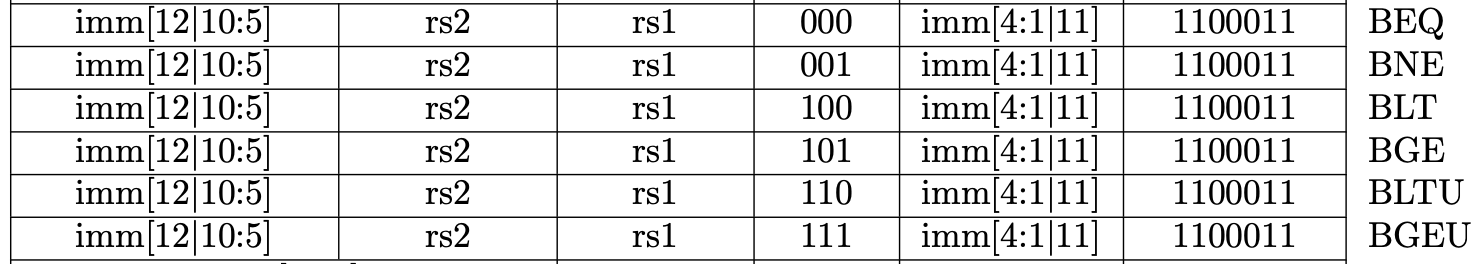
\includegraphics[width=6in,angle=0]{Figures/Fig_Combo_BRANCH_instrs_3}}
  \caption{\label{Fig_Combo_BRANCH_instrs}RISC-V conditional BRANCH instructions}
\end{figure}
The first line just gives us the names of the various slices of a
32-bit BRANCH-type instruction, and the subsequent lines describe the
six instructions.  Note that they only differ in the \verb|funct3|
slice, where they use only six of the possible eight 3-bit codes.

Assuming \verb|instr| is a 32-bit instruction, we can write BSV code
to compute whether \verb|instr| is or is not a legal BRANCH
instruction:

{\small
\begin{Verbatim}[frame=single, numbers=left]
   Bit #(7) opcode_BRANCH = 7'b_110_0011;

   Bit #(7) opcode = instr [6:0];
   Bit #(3) funct3 = instr [14:12];
   Bool legal = (opcode == opcode_BRANCH)
                 && (funct3 != 3'b010)
                 && (funct3 != 3'b011));
\end{Verbatim}
}

Line 1 defines \verb|opcode_BRANCH| as a 7-bit constant whose binary
value is 1100011.  The \verb|`7b| prefix indicates that the number
should be read as a binary, not decimal, number.  The ``\verb|_|''
underscore characters are present merely for our (human) readability,
and have no semantic significance.  Lines 3-4 extract relevant slices,
and finally lines 5-7 define the desired legality condition.

Figure~\ref{Fig_Combo_Is_Legal_BRANCH} shows the hardware circuit described by the code.
\begin{figure}[htbp]
  \centerline{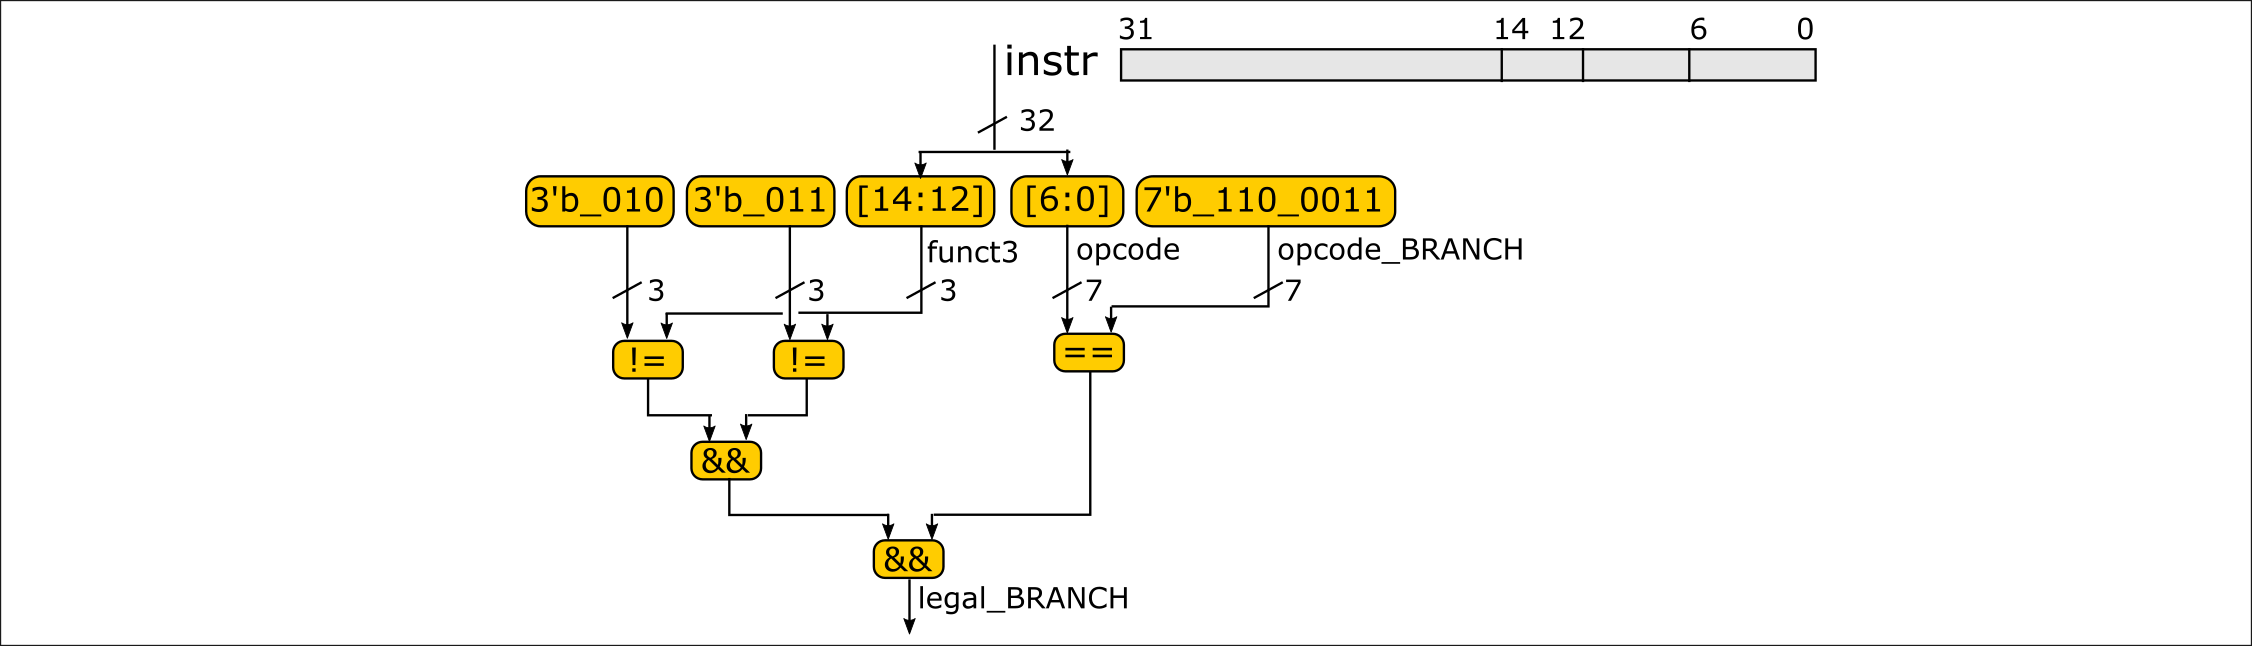
\includegraphics[width=6in,angle=0]{Figures/Fig_Combo_Is_Legal_BRANCH}}
  \caption{\label{Fig_Combo_Is_Legal_BRANCH}Testing for a legal BRANCH instruction}
\end{figure}
Some observations:
\index{BSV!bus (hardware, bundle of wires)}
\begin{tightlist}

 \item Lines with arrow-heads in the figure represent bundles of one
   or more wires, also called ``buses''.  For buses that have more
   than one wire, we show a small diagonal cross-hatch labeled with
   the number of wires (such as ``3'' or ``7'').

 \item Names/identifiers in BSV code that are bound to values are
   simply names for buses (in most software programming languages
   names represent memory locations; this is \emph{not} the case in
   BSV).

\end{tightlist}

% ================================================================

\subsection{Combinational circuits and primitives}

\index{BSV!Combinational circuits}
\index{BSV!Combinational primitives}

Figure~\ref{Fig_Combo_Is_Legal_BRANCH} is an example of a so-called
\emph{combinational} circuit.  In general, a combinational circuit is
any interconnection of combinational primitive ``operators'' that
\emph{does not contain cycles} ({\ie} a bus connecting back to an
earlier part of the circuit).  Examples of combinational primitive
operators in BSV include comparisons (like \verb|==| and \verb|!=|),
boolean operations (like \verb|&&|), bit-slicing (\verb|[n1:n2]|)
truncation and extension, arithmetic (like \verb|+|, \verb|-|,
\verb|*|), shifts (\verb|<<| and \verb|>>|), and multiplexers
(discussed in Section~\ref{BSV_Combo_Circuits_if_then_else}, later).

In BSV, and Verilog/SystgemVerilog RTL, we consider such operators as
``primitive''.  In fact, such operators must themselves be implemented
using lower-level circuit primitives such as AND, OR, and NOT gates
which, in turn, must be implemented with even lower-level circuit
structures such as transistors.  We do not concern ourselves with such
lower-level implementation because nowadays this is performed for us
automatically by excellent so-called ``synthesis'' tools.

% ----------------------------------------------------------------

\subsubsection{Combinational circuits have no side-effects (are ``pure'')}

\index{BSV!Combinational circuits!purity}

There is no ``storage'' in a combinational circuit, nor any concept of
``updating'' any storage (no ``side-effects'').  When a 32-bit value
is presented at the input (top) of the circuit in
Figure~\ref{Fig_Combo_Is_Legal_BRANCH}, conceptually we
``instantly'' see the 1-bit result at the output (bottom) of the
circuit, {\ie} a combinational circuit is conceptually a pure,
instantaneous, mathematical function from intputs to outputs.  If we
change the 32-bit value presented at the input, conceptually the
output changes instantaneously in response.

\index{BSV!Propagation delay}

% ----------------

NOTE: \fbox{\small
\begin{minipage}{5in}

Circuits are physical artefacts and must follow the laws of
physics. Electrical signals will take some finite time to propagate
from inputs to outputs through wires and silicon. This propagation
delay will place a limit on the ``clock speed'' at which we are able
to run a digital circuit.  We ignore this for the moment, and discuss
this in detail later.

\end{minipage}}

% ----------------

% ****************************************************************

\section{Functions}

\label{BSV_functions}

\index{BSV!functions!definition}

The fragments of code shown above can be packaged into BSV functions,
specifying precise types for argument(s) and result:

\input{Code_Extracts/instr_Opcode.tex}
% tag instr_funct3 from line 37, file Instr_Bits.bsv
{\small
\begin{Verbatim}[frame=single, numbers=left, firstnumber=38, label=src\_Common/Instr\_Bits.bsv]
function Bit #(3) instr_funct3 (Bit #(32) instr);
   return instr [14:12];
endfunction
\end{Verbatim}
}

\input{Code_Extracts/is_Legal_BRANCH.tex}

\index{BSV!functions!application}

Functions are invoked using the ``application'' syntax commonly used
in most programming languages:

{\small
\begin{Verbatim}[frame=single, numbers=left]
   Bit #(32) x, y;

   Bool result_x = is_legal_BRANCH (x);
   Bool result_y = is_legal_BRANCH (y);
\end{Verbatim}
}

BSV function definition and application syntax is essentially the same
as in SystemVerilog.

% ================================================================

\subsection{Pure functions vs. functions with side-effects ({\tt Action}, {\tt ActionValue})}

\label{Sec_Pure_vs_Side_Effect_functions}

\index{BSV!Types!{\tt Action}}
\index{BSV!Types!{\tt ActionValue}}
\index{BSV!Action@{\tt Action} type of expression with side-effects}
\index{BSV!ActionValue@{\tt ActionValue} type of experssion with side-effects}

BSV has a system of data types and type-checking similar to Haskell in
that it systematically distinguishes expressions which are ``pure''
(guaranteed not to have any side-effects) from expressions that may
have side-effects.

The detailed reason for this distinction need not detain us
now---suffice it to say here briefly that BSV's semantics are
fundamentally based on a concept of ``rules''; that rules are
condition-action pairs; that conditions \emph{must not} have side
effects (change the state of any hardware); and that the compiler
needs to guarantee this, {\ie} that conditions are pure boolean
expressions.  These points will be discussed in more detail in
Chapter~\ref{ch_Rules_I}.

One useful side-effect during debugging is the {\tt \$display()}
statement.  Why is {\tt \$display()} considered a side-effect?  A pure
expression does not modify any state, and therefore it can be
optimized away by the compiler (evaluated zero times) if its result is
never used.  The compiler can also duplicate a pure expression (so it
is evaluated more than once) for reasons such as cost (cheaper to
recompute a value at some location in the code than to communicate the
value that was computed elsewhere).  Neither of these properties is
true with {\tt \$display()}!  Thus, the compiler needs to know about
the purity or otherwise of every expression.

Keeping track of the purity or otherwise of an expression is not a
local property.  An expression may invoke a function which, in turn,
invokes another function, and so on.  The expression is pure only if
there are no side effects anywhere in such a call chain (those
functions may be defined in separate files, in libraries, and so on).
BSV used a \emph{monadic} type sytem (the same as in Haskell) to
systematically track purity/impurity of expressions.  Consider two
function declarations:

\index{BSV!Haskell, monadic types similarity}
\index{BSV!Monadic types!Haskell similarity}

{\small
\begin{Verbatim}[frame=single, numbers=left]
   function Bool f1 (...); ...

   function ActionValue #(Bool) f2 (...); ...
\end{Verbatim}
}

Both of these functions return a boolean value.  But an application
{\tt f1(x)} is \emph{guaranteed} to be pure (by BSV's type system),
whereas an application {\tt f2(x)} is assumed possibly to have a
side-effect.  These functions also have different syntax for how they
are invoked:

{\small
\begin{Verbatim}[frame=single, numbers=left]
   let result1 = f1 (x);

   let result2 <- f2 (x);
\end{Verbatim}
}

The ``\verb|<-|'' syntax is/can only be used to invoke functions with
\verb|ActionValue| type, and is also a good visual cue to indicate
that the invocation is \emph{performing some action} (side-effect) and
also returns a value.

BSV also has an \verb|Action| type, which is just a convenience for
the special case of an expression that has a side effect and does not
return any interesting value.  You can think of \verb|Action| as a
synonym for \verb|ActionValue #(void)|, where you can think of
\verb|void| as ``uninteresting value''.  For example, you can think of
\verb|$display()| as a built-in function of type \verb|Action|.

% ================================================================

\subsection{Combinational circuits $=$ ``doesn't have {\tt Action} or {\tt ActionValue} type''}

\index{BSV!Combinational circuits!data types}
\index{BSV!Types!of combinational circuits}

Another pleasing consequence of BSV's type system is that we can
identify precisely which expressions become combinational circuits.
If the type of the expression is \emph{not} {\tt ActionValue\#($t$)}
or {\tt Action}, then it \emph{must} be a combinational circuit, and
\emph{vice versa}.

% ================================================================

\subsection{Using {\tt ActionValue} on pure functions for {\tt \$display} debugging}

Sometimes when we write a complex pure function whose result type is
$t$, we may deliberately write its result type as {\tt
ActionValue\#($t$)} so that we can insert \verb|$display| statements
for debugging inside the function body.  If we merely inserted
\verb|$display| statements without changing the function type, the
compiler will complain that the function does not type-check
correctly.

We use this ``trick'' frequently in Drum and Fife source codes, for
tracing and debugging.  We will see many examples in the coming
chapters.

% ****************************************************************

\section{A small testbench to test our code}

\label{BSV_small_testbench}

\index{BSV!Testbenches}
\index{BSV!Testbenches!FSMs}

Here is a small program to run our \verb|is_legal_BRANCH()| function on
a few tests:

\begin{minipage}{6.5in}\small
\begin{Verbatim}[frame=single, numbers=left]
import StmtFSM :: *;

function Bool is_legal_BRANCH (Bit #(32) instr);
   ... as shown earlier ...
endfunction

(* synthesize *)
module mkTop (Empty);

   mkAutoFSM (
      seq
	 action
	    Bit #(32) instr_BEQ = {7'h0, 5'h9, 5'h8, 3'b000, 5'h3, 7'b_110_0011};
	    $display ("instr_BEQ %08h => %0d", instr_BEQ,
		      is_legal_BRANCH (instr_BEQ));
	 endaction

	 action
	    Bit #(32) instr_BNE = {7'h0, 5'h9, 5'h8, 3'b001, 5'h3, 7'b_110_0011};
	    $display ("instr_BNE %08h => ", instr_BNE,
		      fshow (is_legal_BRANCH (instr_BNE)));
	 endaction

	 action
	    Bit #(32) instr_ILL_op = {7'h0, 5'h9, 5'h8, 3'b100, 5'h3, 7'b_110_0000};
	    $display ("instr_ILL_op %08h => ", instr_ILL_op,
		      fshow (is_legal_BRANCH (instr_ILL_op)));
	 endaction

	 action
	    Bit #(32) instr_ILL_f3 = {7'h0, 5'h9, 5'h8, 3'b010, 5'h3, 7'b_110_0011};
	    $display ("instr_ILL_f3 %08h => %0d", instr_ILL_f3,
		      is_legal_BRANCH (instr_ILL_f3));
	 endaction
      endseq);

endmodule
\end{Verbatim}
\end{minipage}

For the moment, don't try to understand all these boilerplate
constructs in detail.  Briefly, \verb|mkAutoFSM| is like a sequential
program (discussed in more detail in Section~\ref{ch_Drum_code}).  It
performs a sequence of four actions.  In each action we define a
32-bit instruction with standard Verilog bit-concatenation syntax.
For example, \verb|instr_BEQ| is defined as a 32-bit value by
concatenating a 7-bit hex 0 as an ``immediate'' value, a 5-bit hex 9
for rs2, a 5-bit hex 8 for rs1, a 3-bit 0 for funct3, a 5-bit hex 7
for rd, and a 7-bit binary value for the branch opcode.
\verb|instr_BEQ| and \verb|instr_BNE| are legal branch instruction
encodings.  \verb|instr_ILL_op| is not a legal branch instruction
because it has the wrong 7-bit opcode in the opcode slice.
\verb|instr_ILL_f3| is not a legal branch instruction because it has
an illegal 3-bit value in the funct3 slice.

In each action, the \verb|$display()| prints the instruction in hex
format, and prints the \verb|Bool| result of applying
\verb|is_legal_Branch()| to the instruction.  In two of the
\verb|$display()|s we print the \verb|Bool| value as a decimal integer
(\verb|%0d| format).  In the other two \verb|$display()|s we use
\verb|fshow()| to print booleans as ``\verb|True|'' or
``\verb|False|''.

Suppose this code is in a file \verb|Top.bsv|.  We can now compile,
link and execute the design (in simulation) as follows:

{\small
\begin{Verbatim}[frame=single, numbers=left]
# ---- Compile BSV source code
$ bsc -u -sim Top.bsv
checking package dependencies
compiling Top.bsv
code generation for mkTop starts
Elaborated module file created: mkTop.ba
All packages are up to date.

# ---- Link to form a simulation exeutable
$ bsc  -sim  -e mkTop -o ./exe_HW_bsim
Bluesim object created: mkTop.{h,o}
Bluesim object created: model_mkTop.{h,o}
Simulation shared library created: exe_HW_bsim.so
Simulation executable created: ./exe_HW_bsim

# ---- Execute the simulator
$ ./exe_HW_bsim
instr_BEQ 009401e3 => 1
instr_BNE 009411e3 => True
instr_ILL_op 009441e0 => False
instr_ILL_f3 009421e3 => 0
\end{Verbatim}
}

% ================================================================

\hdivider

% ----------------
\Exercise

Extend the testbench to test more 32-bit values with
\verb|is_legal_BRANCH()|.

% ----------------
\Exercise

Refer to the ``RV32I Base Instruction Set'' listing in ``Chapter 24
RV32/64G Instruction Set Listings'' in the RISC-V Unprivileged ISA
specification document~\cite{RISCV_Unpriv_2019_12_13}.  It lists 40
RV32I instructions.  Similar to \verb|is_legal_BRANCH()|, write BSV
code for the following functions:

{\small
\begin{Verbatim}[frame=single, numbers=left]
   function Bool is_legal_JAL (Bit #(32) instr);
      ... acccepts JAL

   function Bool is_legal_JALR (Bit #(32) instr);
      ... acccepts JALR

   function Bool is_legal_OP (Bit #(32) instr);
      ... acccepts LUI, AUIPC, ADD, SLT, OR, AND, ...

   function Bool is_legal_OP_IMM (Bit #(32) instr);
      ... acccepts ADDI, SLTI, ..., ORI, ANDI, ...

   function Bool is_legal_Mem (Bit #(32) instr);
      ... acepts LB, LH, LW, LBU, LHU, SB, SH, SW
\end{Verbatim}
}

Ignore FENCE, ECALL and EBREAK instructions; for the moment we'll
treat them as illegal instructions.

% ----------------
\Exercise

Extend the testbench to test more 32-bit values with all the
\verb|is_legal_XXX()| functions.

\Endexercise

% ****************************************************************

\section{{\tt enum} types}

\label{BSV_enum_types}

\index{BSV!enum@{\tt enum} types}

In Figure~\ref{Fig_Instr_Exec}, the Register-Read and Dispatch step
needs to know which of the four alternative downstream paths should be
selected for executing the insruction.  In particular,
we need to know whether the incoming instruction is a system
instruction, a control instruction (branch or jump), an integer
arithmetic/logic instruction, or a memory-accessing instruction.  We
could think of coding these ``classes'' using numbers (0 for system, 1
for control, 2 for integer, 3 for Mem), but it is more readable, and
cleaner, to use an ``enum'' type (similar to enum types in
SystemVerilog and C):

% tag OpClass from line 38, file Inter_Stage.bsv
{\small
\begin{Verbatim}[frame=single, numbers=left, firstnumber=39, label=src\_Common/Inter\_Stage.bsv]
typedef enum {OPCLASS_SYSTEM,     // EBREAK, ECALL, CSRRxx,
              OPCLASS_CONTROL,    // BRANCH, JAL, JALR
	      OPCLASS_INT,
	      OPCLASS_MEM,        // LOAD, STORE, AMO
	      OPCLASS_FENCE}      // FENCE

OpClass
deriving (Bits, Eq, FShow);
\end{Verbatim}
}


This defines a type \verb|OpClass| containing five constants (the last
two (\verb|OPCLASS_MEM| and \verb|OPCLASS_FENCE|) both indicate the
memory-access path.

% ================================================================

\subsection{{\tt deriving (Bits)}}

\index{BSV!deriving Bits@{\tt deriving Bits}}
\index{BSV!Typeclasses}
\index{BSV!Typeclass!instance of}

Because we said ``\verb|deriving(Bits)|'', the \emph{bsc} compiler
will automatically represent them with the obvious codes 0, 1, 2, 3
and 4 in a minimal bit-width (\verb|Bit#(3)|).  If we wanted an
alternative (non-default) coding for these constants, we would
\emph{not} say ``\verb|deriving(Bits)|'', and we would provide an
explicit mapping function into codes (see ``typeclass instances'',
later).

% ================================================================

\subsection{{\tt deriving (Eq)}}

\index{BSV!deriving Eq@{\tt deriving Eq}}

Because we said ``\verb|deriving(Eq)|'', the \emph{bsc} compiler will
automatically define the ``equality'' (and ``inequality'') functions
for values of this new type, in the natural and obvious way (here,
just compare the bit representations for equality).  For other
definitions of equality/inequality, we would \emph{not} say
``\verb|deriving(Eq)|'', and we would instead define
equality/inequality explicitly (see ``typeclass instances'', later).

% ================================================================

\subsection{{\tt deriving (FShow)}}

\index{BSV!deriving FShow@{\tt deriving FShow}}

Given a value \emph{opclass} of type \verb|OpClass|, if we directly
print it, {\eg}:

{\small
\begin{Verbatim}[frame=single, numbers=left]
   opclass = OPCLASS_MEM;
   $display ("opclass = %d", opclass);
\end{Verbatim}
}

the output will be ``3'', which is the numeric code the compiler
assigns to the constant \verb|OPCLASS_MEM| given its position in the
list of labels in the \verb|enum| definition shown in
Section~\ref{BSV_enum_types} (starting at zero).

{\small
\begin{Verbatim}[frame=single, numbers=left]
   opclass = OPCLASS_MEM;
   $display ("opclass = %d", opclass);
\end{Verbatim}
}

Because we said ``\verb|deriving(FShow)|'' in the \verb|enum|
declararion, the \emph{bsc} compiler will automatically define an
``\verb|fshow()|'' function for this type: if we print as follows:

{\small
\begin{Verbatim}[frame=single, numbers=left]
   opclass = OPCLASS_MEM;
   $display ("opclass = ", fshow (opclass));
\end{Verbatim}
}

the output will be ``OPCLASS\_MEM'', {\ie} the symbolic name.

% ****************************************************************

\section{Syntax of Identifiers}

\label{BSV_Syntax_of_Identifiers}

\index{BSV!Identifer syntax}

The syntax of an identifier (name) in BSV follows the same conventions
as in many programming languages: any sequence of alphabets, digits
and underscore characters, with the first letter always being an
alphabet.

\index{BSV!Identifiers!First letter lower- or upper-case}
\index{BSV!Identifiers!Type: initial upper-case letter}
\index{BSV!Identifiers!Enum constant: initial upper-case letter}
\index{BSV!Identifiers!Ordinary: initial lower-case letter}

BSV follows the Haskell system where an identifier has a different
roles depending on whether its first letter is lower-case or
upper-case.  An upper-case first-letter represents a \emph{constant},
either a value constant or a type constant.  All variables (value
variables or type variables) begin with a lower-case letter.

In the enum type-definition in Section~\ref{BSV_enum_types}, the
identifiers \verb|OPCLASS_SYSTEM|, \verb|OPCLASS_CONTROL|,
\verb|OPCLASS_INT| and \verb|OPCLASS_MEM| are all value constants
(they all begin with an upper-case letter).  The identifier
\verb|OpClass| (and identifiers seen earlier: \verb|Bool| and
\verb|Bit|) are all type constants.  The identifiers \verb|Bits|,
\verb|Eq|, and \verb|FShow| are all typeclass constants.

Other variables seen earlier, like \verb|x|, \verb|y|, \verb|a|,
\verb|b|, \verb|opcode|, and \verb|result_x| are all ordinary value
variables.

% ****************************************************************

\section{Syntax of comments}

\label{BSV_Syntax_of_comments}

\index{BSV!Comments!to end-of-line, starting with {\tt //}}
\index{BSV!Comments!block, from {\tt /*} to matching {\tt */}}
\index{BSV!//@{\tt //}, start of comment-to-end-of-line}
\index{BSV!/*@{\tt /*}, start of block comment (until-{\tt */})}

Comments in BSV have the same syntactic conventions as in Verilog,
SystemVerilog and C/C++:

\begin{itemize}

  \item A pair of forward-slashes (``\verb|//|'') begins a comment
    that spans to the end of the current line.

    There are many examples of this in the code fragments already
    shown above.

  \item A region of text spanning multiple lines can be a comment if
    preceded by ``\verb|/*|'' (forward-slash and asterisk) and followed by
    ``\verb|*/|'' (asterisk and forward-slash).

    This form is often used to ``comment-out'' a region of text during
    debugging or trying out alternatives.

\end{itemize}

% ****************************************************************

\section{if-then-else statements and hardware multiplexers}

\label{BSV_Combo_Circuits_if_then_else}

\index{BSV!if-then-else}
\index{BSV!multiplexers}
\index{BSV!MUX}
\index{BSV!multiplexers!cascaded/serial/priority}

In most programming languages, ``if-then-else''` is a so-called
``control'' construct: depending on the boolean condition, either the
then-arm or the else-arm is executed (\emph{not both}!).

In BSV an ``if-then-else`` represents a hardware \emph{multiplexer}.
The then-arm and else-arm each represent hardware that computes some
value.  The if-then-else construct simply selects the output of one of
the two arms and passes it on as its output.  Stated another way, the
if-then-else ``multiplexes'' the two arm-outputs into a single output.
In programming-language terms, \emph{both} arms of the conditional are
always ``executed''---each arm represents an actual piece of hardware
that is continuously computing its output.

The data type of the condition in an if-then-else must always exactly
be \verb|Bool| (not \verb|Bit#(1)|, not an integer, {\etc}).  The
types of the two arms of the conditional must be exactly the same, and
this is also the type of the output of the output of the if-then-else.

For example, here is a function that distinguishes CONTROL
instructions from integer instructions, returning an \verb|OpClass|
(Section~\ref{BSV_enum_types}):

{\small
\begin{Verbatim}[frame=single, numbers=left]
function OpClass instr_opclass (Bit #(32) instr);
   OpClass result;
   if (is_legal_BRANCH (instr)
      || is_legal_JAL (instr)
      || is_legal_JALR (instr))
      result = OPCLASS_CONTROL;
   else
      result = OPCLASS_INT;
   return result;
endfunction
\end{Verbatim}
}

This can also be written using so-called ``conditional expressions''
(using the same syntax as in SystemVerilog and C):

{\small
\begin{Verbatim}[frame=single, numbers=left]
function OpClass instr_opclass (Bit #(32) instr);
   return ((is_legal_BRANCH (instr)
           || is_legal_JAL (instr)
	   || is_legal_JALR (instr))
           ? OPCLASS_CONTROL
	   : OPCLASS_INT);
endfunction
\end{Verbatim}
}

It's a matter of taste and style whether one uses if-then-else
expressions or C-style conditional expressions.  It may also depend on
the size of the sub-epressions.  The primary goal should be
readability.

Both these code fragments represent the same hardware, shown in
Figure~\ref{Fig_Combo_Multiplexer}.
\begin{figure}[htbp]
  \centerline{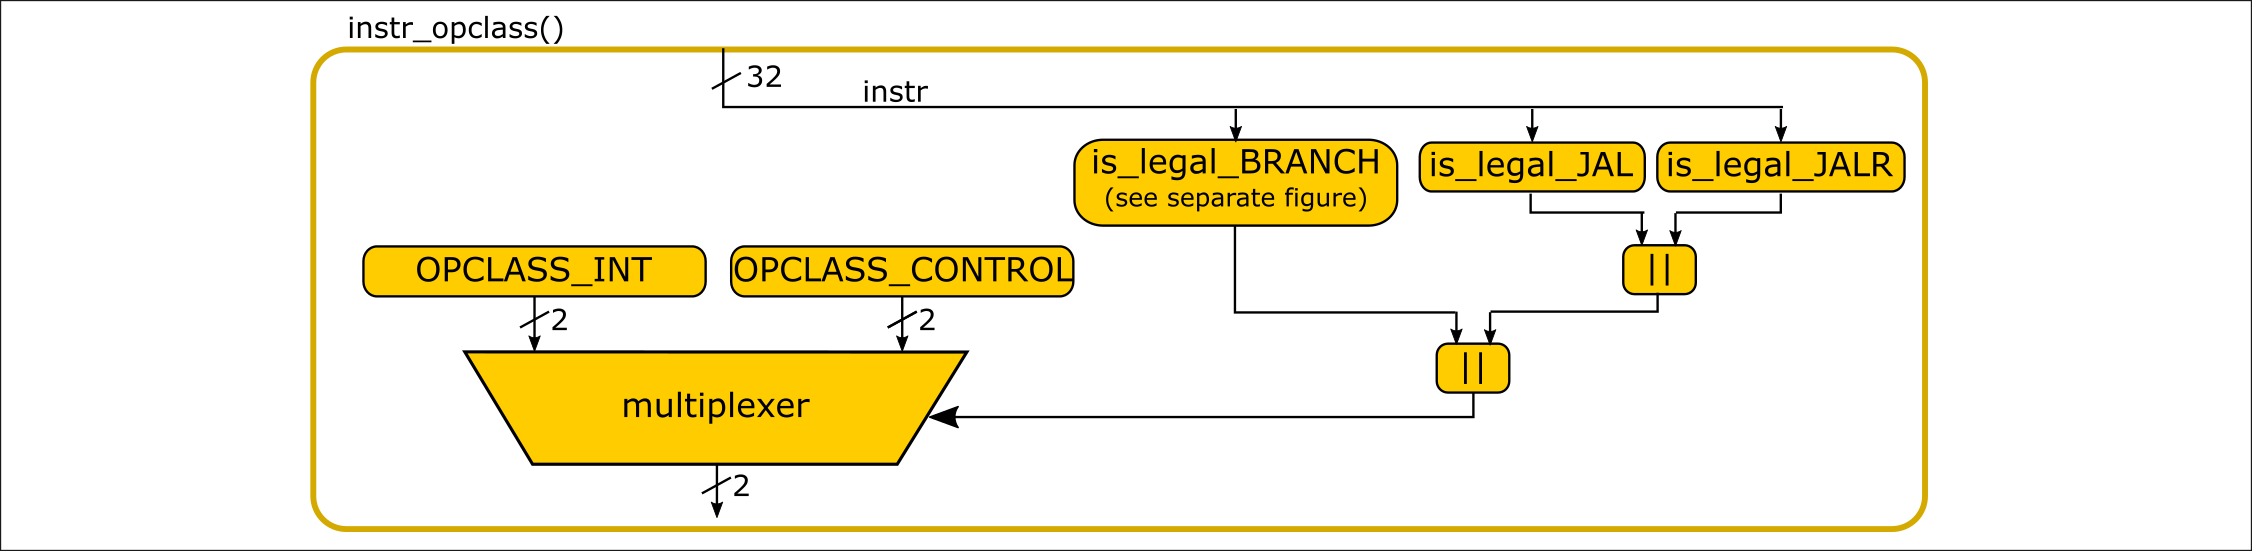
\includegraphics[width=6in,angle=0]{Figures/Fig_Combo_Multiplexer}}
  \caption{\label{Fig_Combo_Multiplexer}If-then-else is a multiplexer}
\end{figure}
The 32-bit \verb|instr| argument is fed into the circuits for
\verb|is_legal_BRANCH()| (hardware schematic in
Figure~\ref{Fig_Combo_Is_Legal_BRANCH}), \verb|is_legal_JAL()| and
\verb|is_legal_JALR()| which are OR'd to produce a \verb|Bool| output
which, in turn, is used to select one of two 2-bit constant values,
producing a final 2-bit result.  The multiplexer, also called a
``MUX'' for short, is a primitive combinational circuit.

If-then-elses and conditional expressions can of course be nested:

\index{BSV!if-then-else!nested}

{\small
\begin{Verbatim}[frame=single, numbers=left]
function Bool instr_opclass (Bit #(32) instr);
   OpClass result;
   if (is_legal_BRANCH (instr)
       || is_legal_JAL (instr)
       || is_legal_JALR (instr))
      result = OPCLASS_CONTROL;
   else if (is_legal_OP (instr)
            || is_legal_OP_IMM (instr)
            || is_legal_LUI (instr)
            || is_legal_AUIPC (instr))
      result = OPCLASS_INT;
   else if (is_legal_LOAD (instr)
            || is_legal_STORE (instr))
      result = OPCLASS_MEM;
   else if (is_legal_ECALL (instr)
            || is_legal_EBREAK (instr)
            || is_legal_MRET (instr)
            || is_legal_CSRRxx (instr))
      result = OPCLASS_SYSTEM;
   return result;
endfunction
\end{Verbatim}
}

This represents a cascade of multiplexers in hardware, as shown in
Figure~\ref{Fig_Combo_Multiplexer_Cascade}
\begin{figure}[htbp]
  \centerline{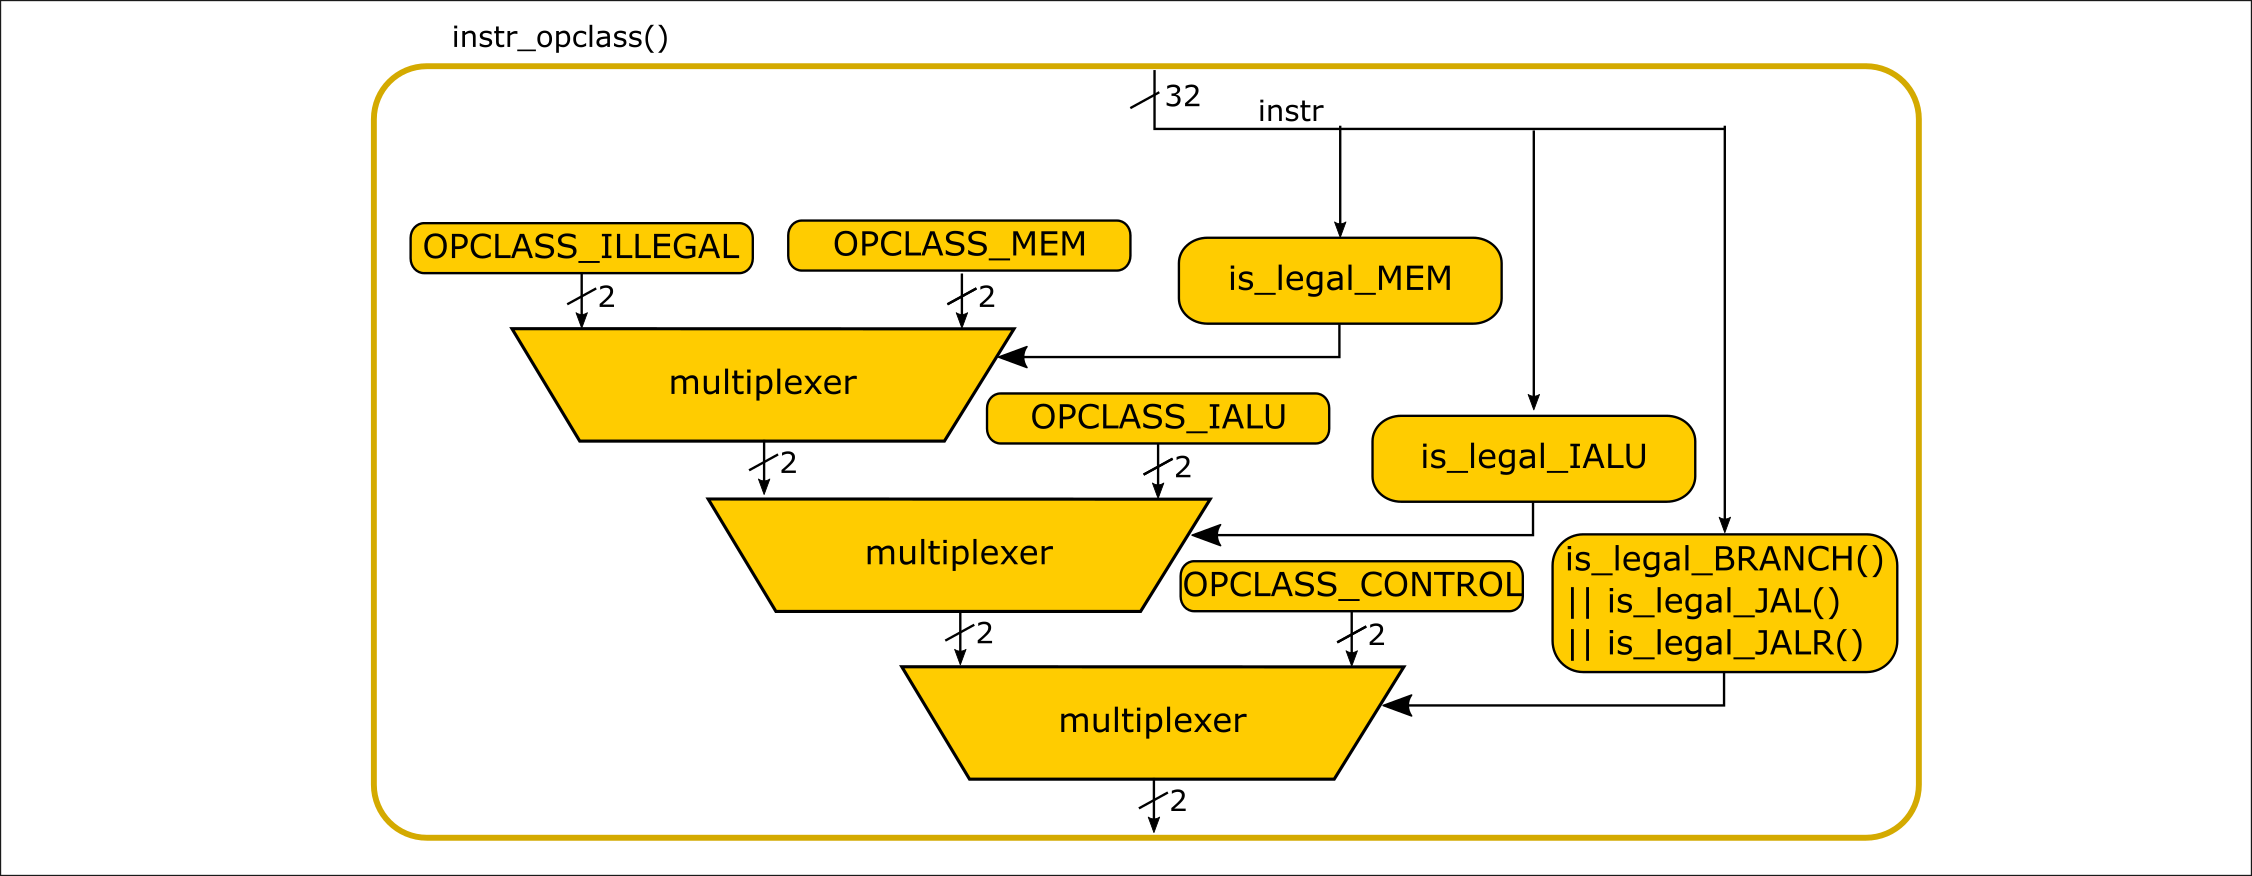
\includegraphics[width=6in,angle=0]{Figures/Fig_Combo_Multiplexer_Cascade}}
  \caption{\label{Fig_Combo_Multiplexer_Cascade}Nested if-then-elses become cascaded multiplexers}
\end{figure}

% ================================================================

\subsection{Parallel multiplexers and MUX synthesis}

\label{Sec_MUXes}

\index{BSV!multiplexers!parallel}

The circuit in Figure~\ref{Fig_Combo_Multiplexer_Cascade} has a serial
structure---the \verb|OPCLASS_CONTROL| branch has priority, and only
if its condition is False can one of the other results flow through.
Also observe that the longest path length increases \emph{linearly}
with number of classes---here, \verb|OPCLASS_SYSTEM| flows through all
four multiplexers.

But we know from RISC-V instruction encodings that the
\verb|OPCLASS_CONTROL|, \verb|OPCLASS_INT| and \verb|OPCLASS_MEM|
conditions are \emph{mutually exclusive}; no instruction
simultaneously falls into more than one such class.  In such
situations (mutually exclusive conditions) it is possible to create
more a efficient circuit called a \emph{parallel MUX}.  An exercise
below shows how to create a parallel MUX explicitly, but in many cases
downstream RTL-to-lower-level-hardware synthesis tools will do this
automatically.

% ================================================================

\hdivider

% ----------------
\Exercise

Write a testbench for the \verb|instr_opclass()| function: pass in
different 32-bit instructions to produce the op class, and print out
the op class.  When printing the class, try printing it as an integer,
and also using \verb|fshow()|.

% ----------------
\Exercise

Write a new version of the \verb|instr_opclass()| function that
expresses a parallel MUX instead of a priority MUX.  The key ideas
are:

  \begin{itemize}

    \item Define a value \verb|x_CONTROL| that is either
      \verb|OPCLASS_CONTROL|, or 0 (of the same bit-width) if the
      \verb|Bool| values of \verb|is_legal_BRANCH()|,
      \verb|is_legal_JAL()| and \verb|is_legal_JALR()| are all False.
      We can implement this by replicating the 1-bit Bool condition to
      the width of the \verb|OpClass| type and bitwise-AND'ing this
      with \verb|OPCLASS_CONTROL|.

    \item Similarly, define values \verb|x_INT| and \verb|x_MEM| that
       is either \verb|OPCLASS_INT|/\verb|OPCLASS_MEM| or 0 if the
       \verb|Bool| value of
       \verb|is_legal_INT()|/\verb|is_legal_MEM()| is False.

    \item Define a value \verb|x_ILLEGAL| that is either
      \verb|OPCLASS_ILLEGAL|, or 0 if any of
      the previous conditions is True.

    \item Finally, just bitwise-OR the four \verb|x_XXX|values
      together to produce there result.

  \end{itemize}

  This kind of MUX is also called an AND-OR mux because of its
  structure.  Note that it relies for correct operation on
  \emph{precisely one} of the bitwise-OR arguments being True.  Here,
  we are assured of this because of the mutual exclusivity of the
  conditions.

% ----------------
\Exercise

Sketch out a schematic diagram for the hardware of the parallel MUX in
the previous exercise.

The schematic will clearly reveal the parallel nature of the MUX
compared to the serial nature of the priority MUX shown earlier in the
schematic in Figure~\ref{Fig_Combo_Multiplexer_Cascade}.

How many multiplexers does each \verb|OPCLASS_XXX| value flow through?
How many bitwise-OR operators are needed?  Note that we can organize
the bitwise-OR operators as a balanced binary tree, so that the path
through the circuit grows \emph{logarithmically}, not linearly, with
the number of classes.

% ----------------
\Exercise

Test your new version of the \verb|instr_opclass()| function in your
testbench.

\Endexercise

% ****************************************************************

\section{Sharing code for RV32 and RV64 {\via} parameterization}

\label{BSV_Paramterizing_XLEN}

\index{BSV!parameterization}

The RISC-V ISA is actually two ISAs---a 32-bit ISA called RV32 and a
64-bit ISA called RV64.  These are not randomly different ISAs; they
have been carefully engineered to overlap as much as possible:

\begin{itemize}

\item Most of the RV32 instructions are exactly the same in RV64

\item Three R32 instructions are slightly different in RV64--the shift
instructions SLLI, SRLI and SRAI have 5-bit shift-amounts in RV32
(allowing up to 32-bit shifts), whereas they have 6-bit shift-amounts
in RV64 (allowing up to 64-bit shifts).

\item RV64 adds several new instructions that compute on 64-bit values.

\end{itemize}

Because of this large overlap of RV32 and RV64, we would like to share
BSV code as much as possible between RV32 and RV64, {\ie} we would
like to parameterize our BSV code so that it can be re-used between
RV32 and RV64 implementations.

% ================================================================

\subsection{Numeric types}

\label{BSV_Numeric_types}

We have mentioned the type \verb|Bit#(n)| frequently so far,
representing bit-vectors of width \emph{n} bits.  All our examples
showed a particular \emph{n}, such as:

{\small
\begin{Verbatim}[frame=single, numbers=left]
   Bit #(32) instr;
   Bit #(32) pc_val;
\end{Verbatim}
}

The first declaration is fine for both RV32 and RV64, since
instructions are 32-bits wide in both.  However, the second
declaration only works in RV32, since the program counter is 64-bits
wide in RV64 (type \verb|Bit#(64)|).

\label{BSV_numeric_types}
\index{BSV!Types!numeric}

The ``32'' or ``64'' argument to the \verb|Bit#(n)| type is a
\emph{numeric type}.  Although syntactically they look just like the
\emph{values} 32 and 64, when used inside a type-expression like
\verb|Bit#(n)|, they are not values, but numeric types.  BSV's
type-system carefully distinguishes between these two cases because
numeric-types usually say something about \emph{hardware structure},
which cannot be changed once created!  So, while we can perform
arbitrary arithmetic on numeric \emph{values}, we cannot do so on
\emph{numeric types}.\footnote{A limited form of arithmetic is
possible on numeric types.  Consider a generic function that takes two
arguments of type {\tt Bit\#(m)} and {\tt Bit\#(n)} and returns the
concatenation of these bit-vectors: its output type is {\tt
Bit\#(m+n)}.  By limiting the available arithmetic \emph{bsc} can
resolve it completely ``statically'', {\ie} at compile time, before it
even compiles to Verilog RTL.  We ignore this for now, and discuss it
later.}

% ================================================================

\subsection{Type synonyms}

\label{BSV_Type_synonyms}

\index{BSV!Types!synonyms}

In BSV we can define a new symbolic name for an existing type, and
then we can use that symbolic names in place of the existing
type. Example, from RV32 code:

{\small
\begin{Verbatim}[frame=single, numbers=left]
   typedef 32 XLEN;      // new name for numeric type 32

   Bit #(XLEN) pc_val;
   Bit #(XLEN) rs1_val;  // Value read from register rs1 in register file
   Bit #(XLEN) rs2_val;  // Value read from register rs2 in register file
   Bit #(XLEN) rd_val;   // Value written to register rd in register file
\end{Verbatim}
}

By changing the single definition in line 1 to:

{\small
\begin{Verbatim}[frame=single, numbers=left]
   typedef 64 XLEN;      // new name for numeric type 32
\end{Verbatim}
}

the remaining code will work for RV64 as well.

% ================================================================

\subsection{The numeric value corresponding to a numeric type}

\label{BSV_value_of_numeric_type}

\index{BSV!valueOf: value of a numeric type}
\index{BSV!Types!valueOf: value of a numeric type}

Although BSV keeps a strict separation of numeric types and numeric
values (and limits the available arithmetic on the former), it is
always safe to convert a numeric type into the corresponding numeric
value, since these values are all known statically (at compile time).
The built-in pseudo-function \verb|valueOf()| is provided for this:

% tag valueOf_XLEN from line 26, file Arch.bsv
{\small
\begin{Verbatim}[frame=single, numbers=left, firstnumber=27, label=src\_Common/Arch.bsv]
Integer xlen = valueOf (XLEN);
\end{Verbatim}
}


Here, \verb|xlen| is an ordinary value variable whose integer value is
the same as that expressed by the numeric type \verb|XLEN|.

% ================================================================

\subsection{Conditional compilation}

\label{BSV_Conditional_compilation}

\index{BSV!Conditional compilation}

Just like in Verilog, SystemVerilog and C/C++, the \emph{bsc} compiler
runs BSV source code through a ``pre-processor'' before compilation,
which can perform simple text (``macro'') substitutions.  Using this
facility, we can pass an argument to the compiler that has the effect
of configuring the source code for RV32 or RV64 (the following code is
from Fife/Drum's \verb|Arch.bsv| file:

% tag XLEN from line 14, file Arch.bsv
{\small
\begin{Verbatim}[frame=single, numbers=left, firstnumber=15, label=src\_Common/Arch.bsv]
`ifdef RV32

typedef 32 XLEN;

`elsif RV64

typedef 64 XLEN;

`endif
\end{Verbatim}
}


As in Verilog and SystemVerilog, pre-processor directives begin with a
\verb|`| character (back-tick) (analogous to \verb|#ifdef| in the
C/C++ pre-processor).

When we invoke the \emph{bsc} compiler, we can pass it command line
arguments \verb|-DRV32| or \verb|-DRV64|; the pre-processor will then
select the appropriate \verb|typedef| line.  Thus, we can write common
code that will work for both RV32 and RV64.  The integer value
\verb|xlen| will have the numeric value 32 or 64 depending on how it
was compiled.

Pre-processor macros allow us to conditionally compile different
source text based on the macro definitions we supply to the compiler.
We can also compile alternatives based on the value \verb|xlen|

{\small
\begin{Verbatim}[frame=single, numbers=left]
   if (xlen == 32) begin
      ... code that must execute if we are in RV32 mode ...
   end
   else begin
      ... code that must execute if we are in RV64 mode ...
   end
\end{Verbatim}
}

Whenever possible, it is preferable to use the \verb|if(xlen==...)|
form instead of the \verb|`ifdef| form for conditional compilation
because (a), the code is more readable and (b), as we experience in
many languages, pre-processor macros can be quite dodgy (scoping,
inadvertant variable capture, inadvertant surprises due to
associativity of infix operators, ...).

Note that in the \verb|if(xlen==...)| form both arms of the
conditional must type-check correctly, whether \verb|xlen| is 32 or
64.  There are ways to achieve this with judicious use of bit-slicing,
\verb|extend()| and \verb|truncate()|; we will point them out as we
encounter them.  If the two arms cannot both type-check whether
\verb|xlen| is 32 or 64, we may have to resort to the \verb|`ifdef|
form.

There is zero run-time overhead in using the \verb|if(xlen==...)| form
because the \emph{bsc} compiler will evalute the if-condition
statically and reduce the if-then-else to just the relevant arm.

% ****************************************************************
